\documentclass{slides}

\setbeamertemplate{footline}[frame number]
\title[What is essential?]{What is essential?}
\subtitle{\footnotesize -- A pilot survey on views about the requirements metamodel of reqT.org}
\author{Björn Regnell}
\institute{Lund University}
\date{March 14, 2016\\ \href{http://refsq.org/2016}{refsq.org/2016}\\ \href{https://github.com/bjornregnell/reqT-survey}{github.com/bjornregnell/reqT-survey}}

\usepackage{xcolor}
\definecolor{entityColor}{RGB}{0,100,200}
\definecolor{attributeColor}{RGB}{0,100,50}
\definecolor{relationColor}{RGB}{160,0,30}

\lstdefinestyle{reqT}{
  %belowcaptionskip=1\baselineskip,
  breaklines=true,
  %showstringspaces=false,
  showspaces=false,
  %breakatwhitespace=true,
  basicstyle=\ttfamily\fontsize{8}{10}\selectfont,
  emph={Ent,Meta,Item,Label,Section,Term,Actor,App,Component,Domain,Module,Product,Release,Resource,Risk,Service,Stakeholder,System,User,Class,Data,Input,Member,Output,Relationship,Design,Screen,MockUp,Function,Interface,State,Event,Epic,Feature,Goal,Idea,Issue,Req,Ticket,WorkPackage,Breakpoint,Barrier,Quality,Target,Scenario,Task,Test,Story,UseCase,VariationPoint,Variant},
  emphstyle=\bfseries\color{entityColor},
  emph={[2]has,is,superOf,binds,deprecates,excludes,helps,hurts,impacts,implements,interactsWith,precedes,requires,relatesTo,verifies},
  emphstyle={[2]\color{relationColor}},
  emph={[3]Attr,Code,Constraints,Comment,Deprecated,Example,Expectation,FileName,Gist,Image,Spec,Text,Title,Why,Benefit,Capacity,Cost,Damage,Frequency,Min,Max,Order,Prio,Probability,Profit,Value,Status},
  emphstyle={[3]\itshape \color{attributeColor}},  
}
\lstset{style=reqT, language=}


\begin{document}

\frame{\titlepage}
\frame{\tableofcontents}

\section{Objective}
\subsection{Research Question}
\begin{Slide}{Research question}
In the context of software requirements engineering education:
\begin{itemize}
\item How to choose a set of \\ \Emph{essential requirements engineering concepts} \\ that allows for \Alert{sufficient expressiveness}, \\ without overloading the metamodel with esoteric concepts just for the sake of \Alert{completeness}?
\pause
\item Presumption: as teachers we should be method agnostic; there is no single ''correct'' dogma
\end{itemize}
\end{Slide}
\subsection{Approach}
\begin{Slide}{Approach}
\begin{itemize}

\item Make a survey among RE scholars
\pause
\begin{itemize}
\item How to quantify ''essentiality''?
\pause
\begin{itemize}
\item One possible quantification: \\ The more scholars that \Emph{agree} on a definition of a concept \\ and \\ the more scholars that \Emph{use} the concept, \\ the more \Alert{essential} is the concept.
\end{itemize}
\end{itemize}
\pause
\item Use the reqT metamodel as a basis for the survey
\end{itemize}
\end{Slide}

\section{Background}
\subsection{About reqT}
\begin{Slide}{What is reqT?}
\begin{itemize}
\item reqT is an open source requirements engineering tool developed in an \Emph{educational} context\\ Download from here: \url{http://reqt.org/} \\ \texttt{java -jar reqT.jar}
\item reqT aims to inspire \Alert{code-loving} cs students to learn more about RE through a \Emph{Scala}-internal DSL
\item reqT has a \Emph{metamodel} including entities, relations and attributes gathered from various sources such as text books, research papers, IREB, wikipedia, etc.
\end{itemize}
\end{Slide}

\begin{Slide}{A small reqT model}
\begin{Code}
val m = Model(
  Feature("chat") has (
    Spec("The system shall enable sending text messages among users"),
    Prio(42)
  )
)
\end{Code}
\end{Slide}

\begin{Slide}{An larger example reqT model}
\begin{Code}
Model(
  Component("appearance") has (
    VariationPoint("color") has (
      Min(0), Max(2), Variant("blue"), Variant("red"), Variant("green")),
    VariationPoint("shape") has (
      Min(1), Max(1), Variant("round"), Variant("square")),
    VariationPoint("payment") has (
      Min(1), Max(2), Variant("cash"), Variant("credit")),
    VariationPoint("payment") requires Variant("cash"), 
    Variant("round") excludes Variant("red"),
    Variant("green") requires Variant("square")),
  Component("appearance") requires VariationPoint("shape"), 
  App("free") has Component("appearance"),  
  App("free") binds (VariationPoint("shape") binds Variant("round")),
  App("premium") has Component("appearance"),  
  App("premium") binds ( 
    VariationPoint("color") binds (Variant("red"), Variant("green")),
    VariationPoint("shape") binds (Variant("round"), Variant("square")),
    VariationPoint("payment") binds Variant("cash")))
\end{Code}
\end{Slide}

\begin{Slide}{49 entities of the metamodel (see paper appendix)}
\fontsize{3.5}{4.0}\selectfont
\begin{tabular}{l l}
\textbf{\textit{Entity}} & \textbf{\textit{Definition}}  \\
\texttt{Actor}&A human or machine that communicates with a system.\\
\texttt{App}&A computer program, or group of programs designed for end users, normally with a graphical user interface. Short for application.\\
\texttt{Barrier}&Something that makes it difficult to achieve a goal or a higher quality level.\\
\texttt{Breakpoint}&A point of change. An important aspect of a (non-linear) relation between quality and benefit.\\
\texttt{Class}&An extensible template for creating objects. A set of objects with certain attributes in common. A category.\\
\texttt{Component}&A composable part of a system. A reusable, interchangeable system unit or functionality.\\
\texttt{Configuration}&A specific combination of variants.\\
\texttt{Data}&Information stored in a system.\\
\texttt{Design}&A specific realization or high-level implementation description (of a system part).\\
\texttt{Domain}&The application area of a product with its surrounding entities.\\
\texttt{Epic}&A large user story or a collection of stories.\\
\texttt{Event}&Something that can happen in the domain and/or in the system.\\
\texttt{Feature}&A releasable characteristic of a product. A (high-level, coherent) bundle of requirements.\\
\texttt{Function}&A description of how input data is mapped to output data. A capability of a system to do something specific.\\
\texttt{Goal}&An intention of a stakeholder or desired system property.\\
\texttt{Idea}&A concept or thought (potentially interesting).\\
\texttt{Interface}&A defined way to interact with a system.\\
\texttt{Issue}&Something needed to be fixed.\\
\texttt{Item}& An article in a collection, enumeration, or series.\\
\texttt{Label}&A descriptive name used to identify something.\\
\texttt{Member}&An entity that is part of another entity, eg. a field in a in a class.\\
\texttt{Meta}&A prefix used on a concept to mean beyond or about its own concept, e.g. metadata is data about data.\\
\texttt{MockUp}&A prototype with limited functionality used to demonstrate a design idea.\\
\texttt{Module}&A collection of coherent functions and interfaces.\\
\texttt{Product}&Something offered to a market.\\
\texttt{Quality}&A distinguishing characteristic or degree of goodness.\\
\texttt{Relationship}&A specific way that entities are connected.\\
\texttt{Release}&A specific version of a system offered at a specific time to end users.\\
\texttt{Req}&Something needed or wanted. An abstract term denoting any type of information relevant to the (specification of) intentions behind system development. Short for requirement.\\
\texttt{Resource}&A capability of, or support for development.\\
\texttt{Risk}&Something negative that may happen.\\
\texttt{Scenario}&A (vivid) description of a (possible future) system usage.\\
\texttt{Screen}&A design of (a part of) a user interface.\\
\texttt{Section}&A part of a (requirements) document.\\
\texttt{Service}&Actions performed by systems and/or humans to provide results to stakeholders.\\
\texttt{Stakeholder}&Someone with a stake in the system development or usage.\\
\texttt{State}&A mode or condition of something in the domain and/or in the system. A configuration of data.\\
\texttt{Story}&A short description of what a user does or needs. Short for user story.\\
\texttt{System}&A set of interacting software and/or hardware components.\\
\texttt{Target}&A desired quality level or goal .\\
\texttt{Task}&A piece of work (that users do, maybe supported by a system).\\
\texttt{Term}&A word or group of words having a particular meaning.\\
\texttt{Test}&A procedure to check if requirements are met.\\
\texttt{Ticket}&(Development) work awaiting to be completed.\\
\texttt{UseCase}&A list of steps defining interactions between actors and a system to achieve a goal.\\
\texttt{User}&A human interacting with a system.\\
\texttt{Variant}&An object or system property that can be chosen from a set of options.\\
\texttt{VariationPoint}&An opportunity of choice among variants.\\
\texttt{WorkPackage}&A collection of (development) work tasks.\\

\end{tabular}
\end{Slide}

\begin{Slide}{28 atributes of the metamodel (see paper appendix)}
\fontsize{6}{6.5}\selectfont
\begin{tabular}{l l}
\textbf{\textit{Attributes}} & \textbf{\textit{Definition}}  \\
\texttt{Benefit}&A characterisation of a good or helpful result or effect (e.g. of a feature).\\
\texttt{Capacity}&The largest amount that can be held or contained (e.g. by a resource).\\
\texttt{Code}&A collection of (textual) computer instructions in some programming language, e.g. Scala. Short for source code.\\
\texttt{Comment}&A note that explains or discusses some entity.\\
\texttt{Constraints}&A collection of propositions that restrict the possible values of a set of variables.\\
\texttt{Cost}&The expenditure of something, such as time or effort, necessary for the implementation of an entity.\\
\texttt{Damage}&A characterisation of the negative consequences if some entity (e.g. a risk) occurs.\\
\texttt{Deprecated}&A description of why an entity should be avoided, often because it is superseded by another entity, as indicated by a 'deprecates' relation.\\
\texttt{Example}&A note that illustrates some entity by a  typical instance.\\
\texttt{Expectation}&The required output of a test in order to be counted as passed.\\
\texttt{FileName}&The name of a storage of serialized, persistent data.\\
\texttt{Frequency}&The rate of occurrence of some entity. \\
\texttt{Gist}&A short and simple description of an entity, e.g. a function or a test.\\
\texttt{Image}&(The name of) a picture of an entity.\\
\texttt{Input}&Data consumed by an entity, \\
\texttt{Max}&The maximum estimated or assigned (relative) value.\\
\texttt{Min}&The minimum estimated or assigned (relative) value.\\
\texttt{Order}&The ordinal number of an entity (1st, 2nd, ...).\\
\texttt{Output}&Data produced by an entity, e.g. a function or a test.\\
\texttt{Prio}&The level of importance of an entity. Short for priority.\\
\texttt{Probability}&The likelihood that something (e.g. a risk) occurs.\\
\texttt{Profit}&The gain or return of some entity, e.g. in monetary terms.\\
\texttt{Spec}&A (detailed) definition of an entity. Short for specification\\
\texttt{Status}&A level of refinement of an entity (e.g. a feature) in the development process. \\
\texttt{Text}&A sequence of words (in natural language).\\
\texttt{Title}&A general or descriptive heading.\\
\texttt{Value}&An amount. An estimate of worth.\\
\texttt{Why}&A description of intention. Rationale.\\

\end{tabular}
\end{Slide}


\begin{Slide}{15 realtions of the metamodel (see paper appendix)}
\fontsize{8}{9}\selectfont
\begin{tabular}{l l}
\textbf{\textit{Relation}} & \textbf{\textit{Definition}}  \\
\texttt{binds}&Ties a value to an option. A configuration binds a variation point.\\
\texttt{deprecates}&Makes outdated. An entity deprecates (supersedes) another entity.\\
\texttt{excludes}&Prevents a combination. An entity excludes another entity.\\
\texttt{has}&Expresses containment, substructure. An entity contains another entity.\\
\texttt{helps}&Positive influence. A goal helps to fulfil another goal.\\
\texttt{hurts}&Negative influence. A goal hinders another goal.\\
\texttt{impacts}&Some influence. A new feature impacts an existing component.\\
\texttt{implements}&Realisation of. A module implements a feature.\\
\texttt{interactsWith}&Communication. A user interacts with an interface.\\
\texttt{is}&Sub-typing, specialization, part of another, more general entity.\\
\texttt{precedes}&Temporal ordering. A feature precedes (is implemented before) another feature.\\
\texttt{relatesTo}&General relation. An entity is related to another entity.\\
\texttt{requires}&Requested combination. An entity is required (or wished) by another entity.\\
\texttt{superOf}&Super-typing, generalization, includes another, more specific entity.\\
\texttt{verifies}&Gives evidence of correctness. A test verifies the implementation of a feature.\\

\end{tabular}
\end{Slide}



\section{Methodology}
\subsection{Data Collection}
\begin{Slide}{Data Collection}
{\centering
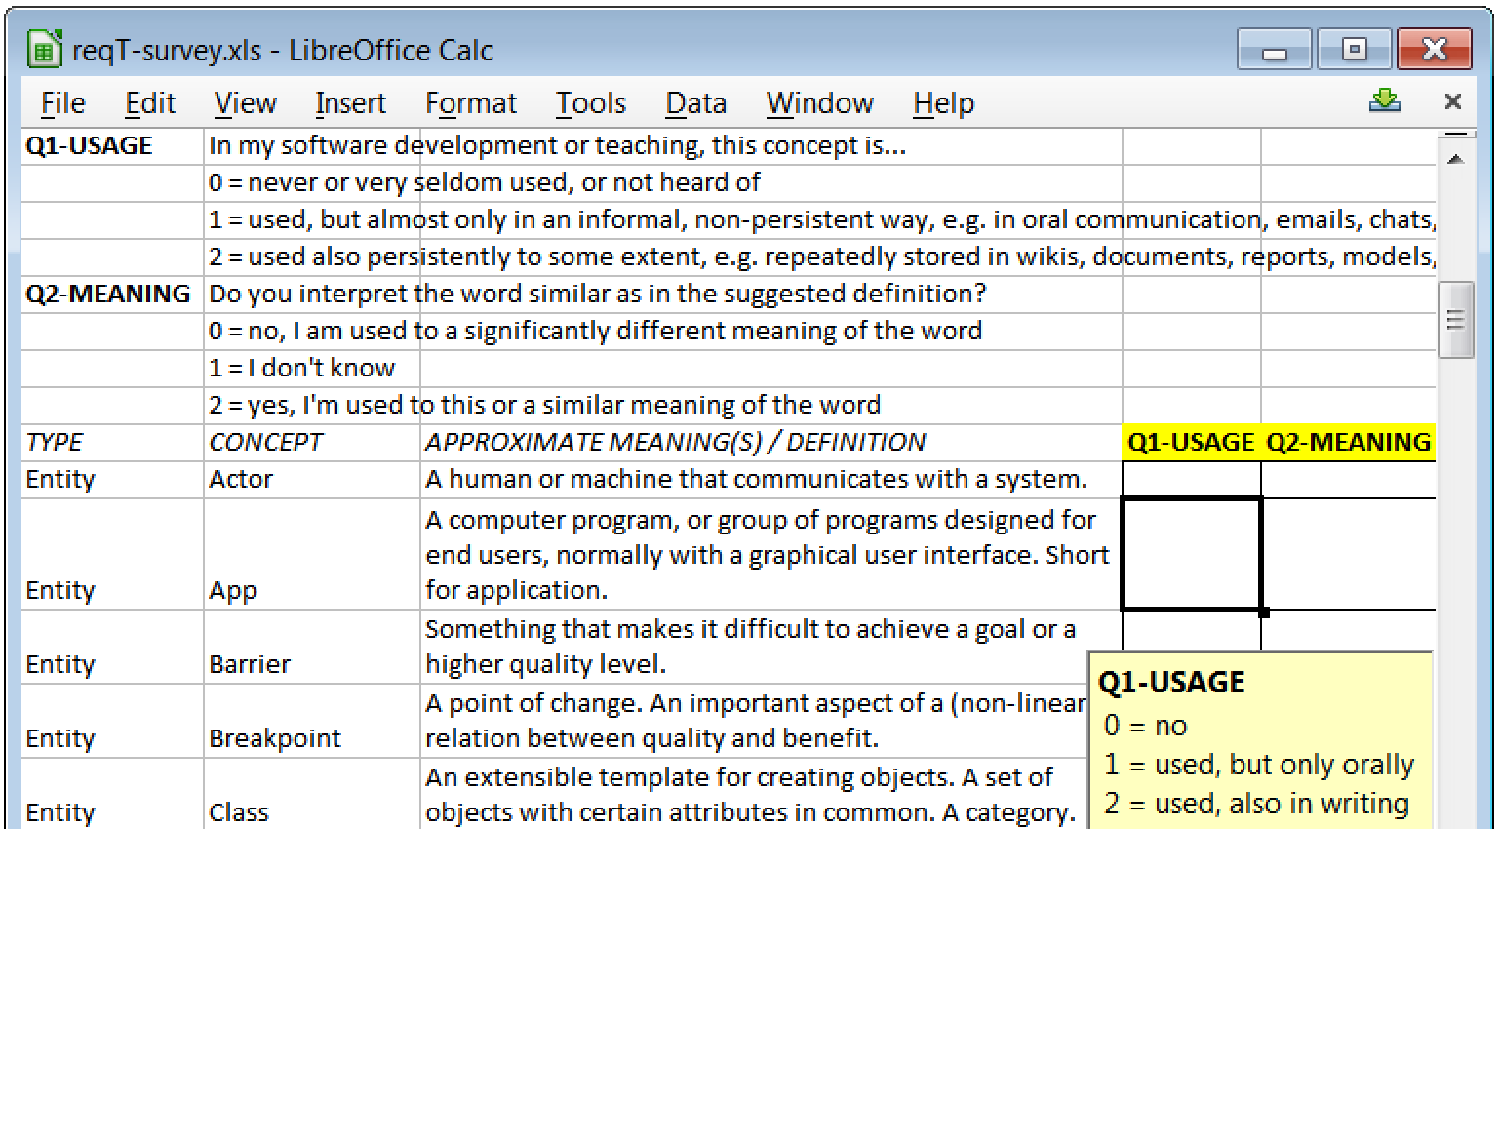
\includegraphics[width=0.8\textwidth]{img/survey-screen-dump}
}
Q1 use? =   no, orally, also in writing\\
Q2 agree? = no, don't know, yes  \\
Answered by 15 swedish RE scholars (100\% response rate)\\
\url{https://github.com/bjornregnell/reqT-survey}


\end{Slide}

\subsection{Data Analysis}
\begin{Slide}{Data Analysis}
\end{Slide}

\section{Results}
\subsection{Essentiality}
\begin{Slide}{Essentiality}
\end{Slide}

\section{Conclusion}
\subsection{Future Work}
\begin{Slide}{Future Work}
\end{Slide}

\end{document}

